%---------------------------------------------------------------------
%
% Chapter 2: Multicriteria Graph Search
%
%---------------------------------------------------------------------
%
% ChapMultiObjAlg.tex
% Copyright 2015 Dr. Francisco J. Pulido
%
% This file belongs to the PhD titled "New Techniques and Algorithms for Multiobjective and Lexicographic Goal-Based Shortest Path Problems", distributed under the Creative Commons Licence Attribution-NonCommercial-NoDerivs 3.0, available in http://creativecommons.org/licenses/by-nc-nd/3.0/. The complete PhD dissertation is freely accessible from http://www.lcc.uma.es/~francis/
%
% This thesis has been written adapting the TeXiS template, a LaTeX template for writting thesis and other documents. The complete TeXiS package can be obtained from http://gaia.fdi.ucm.es/projects/texis/. TeXis is distributed under the same conditions of the LaTeX Project Public License (http://www.latex-project.org/lppl.txt). The complete license is available in http://creativecommons.org/licenses/by-sa/3.0/legalcode
%
%---------------------------------------------------------------------

\chapter{MultiCriteria Graph Search}
\label{chapMultiObjAlg}

%
\begin{FraseCelebre}
\begin{Frase}
It is not the task of the University to offer what society asks for, but to give what society needs.	
\end{Frase}
\begin{Fuente}
Edsger Dijkstra (1930-2002)
\end{Fuente}
\end{FraseCelebre}

This chapter has a twofold purpose, on one hand, provide an overview of two opposite decision paradigms: optimization and satisfaction. On the other hand, deepen insight into the Multicriteria Search Problem (MSP), present the state of the art in algorithms to deal with such problems, and delimit the frame of the algorithms studied in this thesis.

An optimization problem is the problem of finding the best solution from all feasible solutions. This process is suitable for developing computational algorithms that optimize the decision according to given criteria, although in certain cases cannot be appropriate due to its greater computational requirements to solve problems. Humans, however, do not pursue the optimization of their decisions in general. This is where the concept of satisfaction emerges. A satisfactory solution from this perspective is any feasible solution that fulfills the standards or goals of the decision maker. We will further elaborate on both decision paradigms in this Chapter. 

The Multicriteria Decision Making (MCDM) discipline is introduced in the first place in Section \ref{chapMultiObjAlg:sec:MCDM}. Both decision paradigms explained above are part of this discipline. Then, the Multiobjective Optimization Problem (MOP) is presented in Section \ref{chapMultiObjAlg:sec:MOP} along with a classification of the main methods to deal with it. 

Goal Programming (GP), see Section \ref{chapMultiObjAlg:sec:GP}, is a popular method for dealing with multiple objective decision-making problems based on satisfying the goals of a decision maker. GP is a branch of Multicriteria Decision Making that aims to ``satisfice'' instead of optimize. The most popular variants of GP preference modeling are described in Section \ref{chapMultiObjAlg:subsec:GP-variants}. Among them, we focus on Lexicographic GP and introduce relevant definitions concerning this modeling tool in Section \ref{chapMultiObjAlg:subsec:lex-MOP}.

This thesis tackles the Shortest Path Problem with multiple criteria. Prior to defining the MSP, the Shortest Path Problem is defined in Section \ref{chapMultiObjAlg:sec:SPP} along with the most well known approaches to solve it. Right after, the MSP is presented in Section \ref{chapMultiObjAlg:sec:MSP}, as well as a wide range of fields where the MSP has been applied successfully. Sections \ref{chapMultiObjAlg:sec:a-posteriori} and \ref{chapMultiObjAlg:sec:a-priori} analyze the two main algorithmic approaches to solve a MSP, classified depending on the a priori or a posteriori character of the decision maker's preferences. In the first case, we will further study the class of best-first algorithms, and in particular, the state-of-the-art algorithm \namoa. In the second case, we review research on multicriteria search algorithms that can provide compromise solutions or solutions according to some targets.

Finally, Section \ref{chapMultiObjAlg:sec:summary}, summarizes the key concepts of this given chapter, and introduces the motivation and contributions of this research work.

%-------------------------------------------------------------------
\section{Multicriteria Decision Making}
\label{chapMultiObjAlg:sec:MCDM}
%-------------------------------------------------------------------

Multicriteria Decision Making (MCDM), also called Multicriteria Decision Analysis (MCDA), is a sub-discipline of the field of Operations Research. MCDM is a paradigm that involves the consideration of multiple, and in general conflicting, criteria in decision-making environments. In real life problems, there are typically multiple conflicting criteria that need to be evaluated in making decisions. The purpose of MCDM is to support decision makers (an individual or a group of individuals) to make those decisions. Typically, there does not exist a unique optimal solution for such problems and it is necessary to use the decision maker's (DM) preferences to select between solutions. For instance, when buying a new computer, cost, performance and design may be some of the main criteria a buyer considers. It is unusual to have the cheapest computer to be the best designed and the most powerful. 

%According to Dr. Carlos Romero, a formal definition of MCDM is: "Set of mathematical methods and computational techniques that with an explicative, normative or prescriptive purpose, aim to assess a finite and explicite (discrete case) or an infinite number of alternatives based upon a finite number of criteria"

Solving a MCDM problem can be interpreted in different ways. A decision maker can seek the "most preferred" alternative, i.e. the best alternative from a set of available alternatives. Another interpretation could be choosing a small set of good alternatives, or grouping alternatives into different preference sets. Finally, the last interpretation could be to find all \textit{efficient} or \textit{non-dominated} alternatives. 

Let us first introduce some relevant concepts taken from \citep{Romero1991,Romero1993}: 

\begin{defi}\label{defi:attribute}
Zeleny \citep{Zeleny1982} and Romero define \textbf{attributes} as descriptors of an objective reality to represent values of the DMs. These values are measurable properties that can be expressed as a mathematical function $g(\vec x): X \rightarrow \mathbb{R}$, where $\vec x$ is the vector of the decision variables and $X$ is the set of solutions to the decision problem. 
\end{defi}

\begin{defi}\label{defi:objective}
\textbf{Objectives} represent the desired improvement of an attribute, i.e. the maximization or the minimization of the mathematical functions corresponding to the attributes under consideration. In short, objectives take the form: $\max g(\vec x)$ or $\min g(\vec x)$.
\end{defi} 

\begin{defi}\label{defi:targetgoal}
A \textbf{target} or aspiration level, $t \in \mathbb{R}$, is an acceptable level of achievement for any of the attributes considered by the DM. A \textbf{goal} is a combination of an attribute with a target, stated by the decision maker to define their preference. 
\end{defi}

\begin{defi}\label{defi:deviation}
A \textbf{deviation variable} represents the distance between the \textit{i-th} goal and its associated aspiration level. A formulation model is defined as the minimization of the deviation variables to achieve the goals. Three different kinds of goals are defined in this context. In each of them we select different deviation variables to minimize. Table \ref{tab:deviation-variables} shows the concept of unwanted deviation variable, or variable to minimize, depending on the kind of goal.

\begin{table}
\caption{Goals and deviation variables (taken from \citep{Romero1993}.}
\centering
\begin{tabular}{ccc}
\hline \noalign{\smallskip}
Type of objective function & Goal type & Deviation to minimize\\
\noalign{\smallskip} \hline
Minimization & $g_i(\vec x) \leq t_i$ & $d_i$ \\
Maximization & $g_i(\vec x) \geq t_i$ & $p_i$ \\
Exact achievement & $g_i(\vec x) = t_i$ & $d_i + p_i$ \\
\hline
\end{tabular}
\label{tab:deviation-variables}
\end{table}  

The distance between the \emph{i-th} goal and its associated aspiration level may be negative (represented by $d_i$) or positive (represented by $p_i$). A negative value represents the number of units in which the \textit{i-th} goal falls below with respect to the target defined. The positive value represents just the opposite, i.e. the number of units in which the achievement of the \textit{i-th} goal has been surpassed regarding the aspiration level proposed. In general, the \textit{i-th} goal expressed algebraically is, 
\begin{equation}\label{eq:goal-mat}
g_i(x) + d_i - p_i = t_i \qquad d_i, p_i \geq 0
\end{equation}
\end{defi}

\begin{defi}\label{defi:criterion}
The term \textbf{criterion} comprises attributes, objectives and goals of a DM relevant to a particular decision-making problem.
\end{defi}

\citet{Romero1993} splits the MCDM framework into two scenarios. The first one corresponds to a decision making situation with a discrete number of feasible solutions to be ranked according to different attributes. In this case a multiattribute utility function represents the preferences of the DM and is used to order the set of finite feasible alternatives. This approach is called Multiattribute Decision Making (MADM) (see for example \citep{tzeng2011}).

The second scenario corresponds to a decision making situation with an infinite number of decision alternatives where the practical possibility of obtaining a reliable representation of the DM's utility function is very limited. In this case with multiple objectives the Multiobjective Optimization, also known as  Multiobjective Programming (MOP), is the approach to consider. In general, a Multiobjective Optimization problem assumes a simple preference structure, the so-called Pareto ordering \citep{Pareto1897}, to find the set of trade-offs between all objectives considered \citep{ChankongHaimes1983}.

Let us now revise a formal definition of the Multiobjective Optimization Problem, introduce definitions relevant to this research work, and classify the most popular techniques to deal with it.

%-------------------------------------------------------------------
\section{Multiobjective optimization}
\label{chapMultiObjAlg:sec:MOP}
%-------------------------------------------------------------------

Let us first introduce a mathematical formulation of the Multiobjective Optimization Problem, 

\begin{defi}\label{chapMultiObjAlg:def:multiObjProb}
Let $X$ be the set of feasible solutions to a problem and let $f^k:X \rightarrow \mathbb{R}$ be $k$ functions assigning a real value as image to a solution in $X$, being $k \in \{1,2,\ldots ,q \}$ objectives. A multiobjective problem in $X$ can be formulated as a minimization problem,
\begin{eqnarray}\label{chapMultiObjAlg:eq:probMultiObj}
     \min \vec f(\vec x)=(f^1(\vec x),f^2(\vec x),\ldots ,f^q(\vec x)) \\
\nonumber \raggedleft	  s.t. \ \vec x \in X
\label{chapMultiObjAlg:eq:probMultiObj2}
\end{eqnarray}
\end{defi}

Note that there is no loss of generality in considering the objective function's minimization, since the maximization case can be reduced to this one. The criteria to be minimized are the so-called \textbf{objectives}. In general, there is not a single solution to the multiobjective problem which is simultaneously optimal for all objective functions. Hence, in this context the concept of optimality is replaced by the concept of Pareto optimality, and the solutions to a multiobjective problem are called \textbf{Pareto-optimal}, non-dominated or \textbf{efficient solutions}. 

\begin{defi}\label{defi:Pareto-solution}
A particular solution to a Multiobjective Optimization Problem is said to be \textbf{Pareto-optimal} or \textbf{Pareto-efficient} if no other solution to the problem can improve according to one objective without worsening at least one of the others.
\end{defi}

\begin{defi}\label{defi:Pareto-set}
The set of solutions to a Multiobjective Optimization Problem, known as \textbf{efficient set}, \textbf{Pareto frontier} or \textbf{Pareto set}, comprises all the feasible Pareto-optimal solutions to the problem.
\end{defi}

The main difference between a Multiobjective Optimization Problem and its scalar counterpart is the use of cost vectors which induce only a partial order relation. We will now reproduce some standard definitions regarding preference relations between $q$-dimensional cost vectors $\vec y, \vec{y'} \in \mathbb{R}^q$.

\begin{defi}\label{chapMultiObjAlg:def:dominance}
A partial order relation $\prec$ denominated \textbf{dominance} or Pareto-optimal preference is defined as follows:

\begin{equation}
\vec{y} \prec \vec{y'} \quad
\Leftrightarrow \quad
\forall i \ (1\leq~i\leq~q) \quad y_i \leq y'_i \ \land \ \vec{y} \neq \vec{y'}
\end{equation}
\end{defi}
and we define equivalently the preference relation  $\preceq$ called \emph{dominance or equality}
\begin{eqnarray}
\forall \vec y,  \vec{y'} \in \mathbb{R}^q \quad
\vec y \preceq  \vec{y'} \quad
\Leftrightarrow \quad
\vec y \prec \vec{y'} \ \ \lor \ \ \vec y = \vec{y'}
\end{eqnarray}
where $y_i$ denotes the i-th component of vector $\vec y$.

Therefore, given two $q$-dimensional vectors $\vec y$ and $\vec{y'}$ (where $q > 1$), it is not always possible to say that one is preferred to the other. For instance, in a three-dimensional cost space, vector $(2,3,1)$ dominates $(5,6,3)$ and $(3,6,4)$ but no dominance relation exists between $(2,3,1)$ and $(1,7,3)$ or $(5,2,7)$. They are all said to be \emph{non-dominated}. 

\begin{figure}
\centering
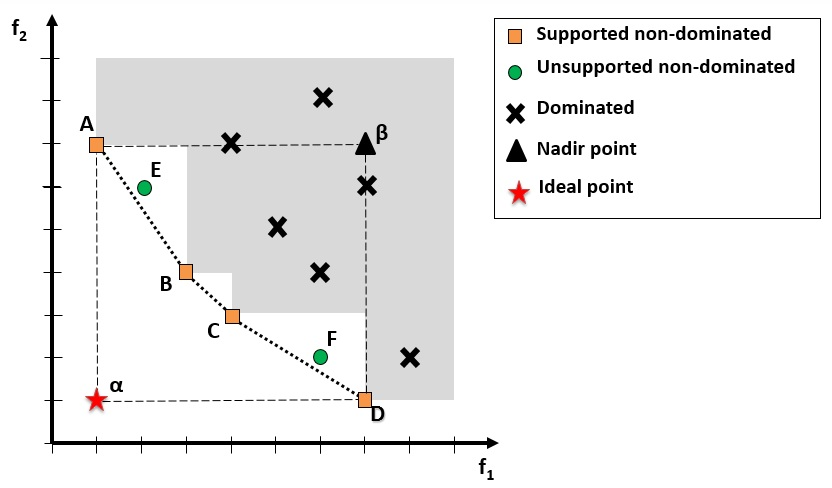
\includegraphics[width=1\textwidth]{Images/Chapter2/MOP-solutions}
\caption{Types of solutions and relevant points in a biobjective cost space.}
\label{fig:2-1}
\end{figure}

The Pareto-optimal solutions to the minimization problem can be split into two different types:
\begin{description}
    \item[Supported] They can be obtained as optimal solutions to a single-objective weighted sum problem (WSP). For instance, for the biobjective case (i.e. $q=2$), where $\vec x=(x_1,x_2)$, these include all optima of the following function, for all values of the $\lambda_1$ and $\lambda_2$ parameters.
\begin{equation}\label{chapMultiObjAlg:eq:wsp}
    \min_{x\in X} \lambda_1 x_1 + \lambda_2 x_2
\end{equation}
The set of all supported efficient solutions is denoted by $X_{S}$, and the set of non-dominated image values by $F_{S}$. 
    \item[Unsupported] The remaining non-dominated solutions are called \textit{unsupported} solutions. They cannot be obtained as solutions to WSPs. Unsupported solutions are located in the interior of triangles formed by two adjacent supported solutions. These areas are denominated \textit{duality gaps} by some authors. 
\end{description}

Let us take a look at Figure \ref{fig:2-1}, where a sample bidimensional image space is depicted. Points $A=(1,7)$, $B=(3,4)$, $C=(4,3)$,  and $D=(7,1)$ represent supported solutions. The \textit{extreme} non-dominated solutions are supported solutions that have the minimum possible value in at least one of the objectives (points $A$ and $D$). Points $E=(3,5)$ and $F=(6,2)$ represent unsupported non-dominated solutions. 

\begin{defi}\label{chapMultiObjAlg:def:nondom}
Given a set of vectors $X$, we shall define $\mathcal{N}(X)$ as the \textbf{set of non-dominated vectors} in $X$ in the following way:

\begin{equation}
  \mathcal{N}(X) = \{\vec x \in X \  | \  \nexists \vec y \in X \quad \vec y \prec \vec x\}
\end{equation}

\end{defi}

\begin{defi}
We say that a vector $\vec x$ is dominated by a set $X$ when 
there exists $\vec{x'}\in X$ such that $\vec{x'} \prec \vec x$. Thus, all points represented as crosses in Figure \ref{fig:2-1} are dominated by ${N}(X) = \{ (1,7) , (3,4), (4,3), (7,1) \}$.
\end{defi}

\begin{defi}\label{chapMultiObjAlg:def:idealnadir}
Let us denote $\alpha_i = min_{\vec x \in \mathcal{N}(X)}\{x_i\}$, and
$\beta_i = max_{\vec x \in \mathcal{N}(X)}\{x_i\}$. The set $\mathcal{N}(X)$ is bounded by the \textbf{ideal point} $\vec \alpha = (\alpha_1 \ldots \alpha_q)$,
and the anti-ideal or \textbf{nadir point} $\vec \beta = (\beta_1 \ldots \beta_q)$. The ideal point can be calculated optimizing each objective separately. However, for $q > 2$ it is difficult to calculate the nadir point without computing the whole set of non-dominated solutions. 
\end{defi}

In Figure \ref{fig:2-1} the ideal and nadir points are represented as a red star and a black triangle, respectively. The set $\mathcal{N}(X)$ is bounded by the extreme non-dominated solutions A and B, the ideal point ($\alpha$) and the nadir point ($\beta$).

Since there usually exist multiple Pareto-optimal solutions for Multiobjective Optimization Problems, there are different approaches in the literature to the concept of "solving a Multiobjective Optimization Problem". This concept is often understood as approximating or obtaining all or a representative set of Pareto-optimal solutions \citep{ehrgott2005}. Approaches can be also divided into those methods providing approximate solutions, and those providing exact solutions. 

There is a great variety of approximate techniques applied to the Multiobjective Optimization Problem e.g. fuzzy, and metaheuristics. Within them we can find a large amount of approaches like genetic algorithms, tabu search, or ant colony systems to name a few. A classification of all types of approaches to solve MOP is out the scope of this thesis. Some classifications can be found in \citep{Ehrgott2000,ehrgott2005,Branke2008}.   

Some popular exact approaches combine multiple objectives into one single objective. The most used one is the weighted sum or scalarization method. This method along with Multiobjective Linear Programming (MOLP) is often included within the exact algorithms, although only the set of supported solutions can be found. 

To classify exact algorithms that tackle the MOP we follow the general classification of MCDM methods, which can also be extended to MOP, proposed and followed by different authors over the years \citep{cohon1978,climacopascoal2012}. The following categories distinguish the methods according to the role of the decision maker in the resolution process: 

\begin{enumerate}
	\item \textbf{A priori methods}. The first category comprises those methods in which the preferences of the DM have been provided a priori. These preferences might be given for instance in the form of an utility function or goals to satisfy. Compromise Programming (CP) and Goal Programming (GP) are the most popular techniques included in this category. Some authors also believe than GP could be included in the next category \citep{Jones2010}, since it can be correctly used as a part of the interactive process to develop and refine the model accurately to reflect the decision maker preferences. 
	\item \textbf{Interactive decision process}. The decision maker can also be involved directly in the solution process. The methods which lie in this category establish a dialogue between the DM and the algorithmic resolution. If the DM is satisfied with the non-dominated solution provided, the algorithm finishes; otherwise, the calculation phase continues and the DM may set new preferences.
	\item \textbf{A posteriori methods}. The third category includes methods where a multiobjective analysis is performed. There are no preferences given by the decision maker and therefore, the whole set of efficient solutions must be calculated. Afterwards, this set is analyzed by the decision maker. It is worth mentioning that returning the whole Pareto frontier can be a computationally costly procedure. Therefore, these methods may have prohibitive runtimes when they are applied to large problems.
 
\end{enumerate}

The two mentioned a priori approaches are MCDM distance function methods. Actually, both methodological approaches aim to minimize the distance, not in a geometric sense but in a preferential one, between a certain point and the actual achievement for each of the objectives under consideration. This point is represented in GP as a set of targets. Analogously, CP uses the \emph{ideal point} (Definition \ref{chapMultiObjAlg:def:idealnadir}) which corresponds to the optimum value of each objective. 
%Finally, RPM represents this point as a reference level which plays the role of a control tool to be used in a mobile manner by the decision maker (DM) \citep{Romero1998}.

Let us now turn our attention to the Goal Programming methodology.

%-------------------------------------------------------------------
\section{Goal Programming}
\label{chapMultiObjAlg:sec:GP}
%-------------------------------------------------------------------

Goal programming is one of the oldest and most successful multicriteria decision making techniques \citep{ChankongHaimes1983}. GP was born in the beginning of the 1960s thanks to the contributions of \cite{Charnes1961}. Many variants and an impressive number of applications followed, enumerating hundreds of papers dealing with a wide range of problems and applications \citep{Ignizio1976, Ignizio1978, Ignizio1984, Charnes1977, Zeleny1981, Zeleny1982, Zeleny1984, Zanakis1985, Romero1986, Romero1991, Schniederjans1995, Tamiz1998, Aouni2001}. Several surveys have also been recently presented to review the improvements in the field \citep{Caballero2010,Orumie2014, Aouni2014}. 

Currently, GP has evolved from its original form into a powerful methodology that may incorporate techniques from artificial intelligence, such as genetic algorithms \citep{Pal2012, Deb1999} or fuzzy logic \citep{Bankian-Tabrizi2012, Shahnazari-Shahrezaei2013, Sen2013, DaSilva2014}. 
%or multicriteria search \citep{Mandow2001, Mandow2013, Pulido2014}.

Two key concepts serve to distinguish GP from conventional methods of optimization. First, the use of goals, or flexible constraints, as opposed to the rigid constraints of single objective optimization in mathematical programming, and second, the philosophy of ``satisficing'' as opposed to optimizing. The term satisfice was introduced by \citet{simon1956} as a combination of the terms satisfy and suffice. 

As a consequence of the principle of satisficing, any solution to a goal programming problem is ranked by an achievement function which measures the degree of deviation from the problem goals when these goals can not be satisfied. The specific way in which this deviation is measured characterizes the particular model of the GP approach that is employed.

It must be emphasized that, despite the popularity of the GP model, a weakness have been pointed out from the DM point of view. In general, GP methods do not guarantee that the obtained solution is Pareto-optimal, though some tests of Pareto optimality can be found in \citet{Miettinen1999, Larbani2007}. 
%This thesis is focused on the combination of the Multicriteria Search with goal-based preferences where all the algorithms proposed and analyzed in it return Pareto optimal solutions, regardless whether the goals can be satisfied or not. 

%-------------------------------------------------------------------
\subsection{Variants of goal-based preferences}
\label{chapMultiObjAlg:subsec:GP-variants}
%-------------------------------------------------------------------

Section \ref{chapMultiObjAlg:sec:MCDM} introduced the concepts of attribute, objective, target and deviation variables. Following those concepts, we introduce below the most popular GP formulation models. At this point, it is important to mention that inequalities have been traditionally used in mathematical programming models to define the set of feasible solutions to a problem. From a mathematical point of view, goals and constraints share the same syntax. However, their semantics are quite different. Constraints must be satisfied by candidate solutions to be acceptable. If all constraints cannot be simultaneously satisfied, the problem is inconsistent and there is no solution. Goals, on the other hand, are used to represent the decision maker's preferences. They represent their desires or aspirations. Hence, feasible solutions may or may not achieve all goals. A solution to a goal problem is \emph{satisfactory} when \emph{all} the goals can be satisfied. If there are no satisfactory solutions to a problem, GP seeks solutions that minimize deviation from the targets.

\cite{Romero1991} divides GP formulations in two categories. Both GP formulations do not generate the same solution, neither is one method superior to the other, because each variant is designed to satisfy certain decision makers' preferences. 

\begin{enumerate}

    \item \textbf{Weighted Goal Programming (WGP)}.
The first approach, called weighted goal programming (WGP), considers all goals simultaneously as they are all in a composite objective function. This function aims to minimize the sum of all the deviations between the goals and their aspirational levels. The deviations are weighted according to the relative importance of each goal for the DM.

In WGP weights are associated to each of the goals to establish the relative importance of deviations from their target. WGP handles several goals simultaneously by adding their relative deviations, hence, a normalization of constants is generally required in this model. Popular choices to normalize deviations are the goal target values (hence turning all deviations into percentages) or the range of the corresponding attribute (between the best and the worst possible values, hence mapping all deviations onto a zero-one range).

    \item \textbf{Lexicographic (or pre-emptive) Goal Programming (LGP)}.
The second approach, called pre-emptive or lexicographic goal programming (LGP), requires ranking all the goals in order of importance. The different goals are divided into several levels of pre-emptive priorities in such a way that if a specific priority level $Q_i$ is preferred to another priority level $Q_{i+1}$, then the fulfillment of the goals in $Q_i$ is infinitely more important than the fulfillment of the goals in $Q_{i+1}$. 

This variant models a problem with a combination of both weighted and lexicographic approaches. This model can suit the decision maker preferences when the attributes can be categorized into groups where the attributes within a group $k$ are infinitely more important to satisfy than those of level $k+1$. Each level can have one or more attributes and their importance within the level is established by a certain weight also defined by the DM. 
\end{enumerate}

We further analyze lexicographic goal-based preferences in the next section.

%-------------------------------------------------------------------
\subsection{Lexicographic goal-based preferences}
\label{chapMultiObjAlg:subsec:lex-MOP}
%-------------------------------------------------------------------

This section introduces a formal characterization of lexicographic goal-based preferences that will be later used in our formulation. Let us first recall that Goal Programming is a distance function method, that is, it aims to minimize the distance or deviation from the actual solution achievement to the point that represents the goals established by the DM. Therefore, the way to define and measure this deviation is an important component of the GP model. Let us now consider a problem, where goals are always of the form $g_i(\vec x) \leq t_i$. Let $\vec g = (g_1,g_2,...,g_q)$ be a vector of $1 \leq i \leq q$ attributes (costs) of a given solution $\vec x \in X$. Several methods have been proposed to measure the deviation of a solution vector from a set of goals. The most frequent ones are the following \citep{Romero1991, Romero1993}: 

\begin{itemize}
   \item minimization of the weighted sum of deviations: 
\begin{equation}\label{eq:deviation}
   d(\vec{g}) = \sum_{i=1}^{q} w_{i} \times \max(0, g_{i} - t_{i}), 
\end{equation}
	\item minimization of the maximum weighted deviation, also called minmax strategy:
\begin{equation}\label{eq:deviation-maxmin}
   d(\vec{g}) = \max_i[w_{i} \times \max(0, g_{i} - t_{i})].
\end{equation}
\end{itemize}

Notice that this definition measures the deviation of the vector $g$ with respect to the set of targets defined by the DM, i.e. corresponds to the aggregation of the non-achievement values of each individual goal $g_{i} - t_{i}$ (see Definition \ref{defi:deviation}). We do not consider deviation when a goal is satisfied. 

In the lexicographic goal-based model formulation we introduce below, we build upon the deviation measured as the minimization of the weighted sum of deviations. Let $\vec g = (g_1,g_2,...,g_q)$ be a vector of $1 \leq i \leq q$ attributes of a given solution $\vec x \in X$, where $g_i: X \rightarrow \mathbb{R}, 1 \leq i \leq q$ grouped in $l$ priority levels sorted in order of decreasing preemptive importance. Each priority level $k$ comprises a set $I_k$ of one or more attributes. Goals are defined by setting \emph{targets} $t_i$ for each attribute, always in the form $g_{i}(x) \leq t_{i}$.

This model considers the minimization of the weighted sum of deviations for each priority level, i.e. we measure the deviation of a solution vector from a set of goals grouped in preemptive priority levels of importance. We can calculate a deviation vector for $\vec g$ with one component for each priority level, $\vec{d}(\vec{g}) = (d_1(\vec{g}), d_2(\vec{g}),..., d_l(\vec{g}))$. For each level $k$, its deviation $d_k$ can be defined as:

\begin{equation}\label{eq:deviation-lex}
   d_k(\vec{g}) = \sum_{i\in I_k} w_{i} \times \max(0, g_{i} - t_{i})  
\end{equation}
where $w_i$ is the relative weight of goal $i$ in level $k$.

Let us now introduce some more relevant preference relations between vectors that will be employed throughout this research work.

\begin{defi}\label{chapMultiObjAlg:def:lexorder}
Let us consider two $q$-dimensional vectors $\vec y, \vec{y'} \in \mathbb{R}^q $. A total order relation $\prec_{L}$ denominated \textbf{lexicographic order} is defined as follows: 
\begin{equation}\label{chapMultiObjAlg:eq:lexorder}
 \vec{y} \prec_{L} \vec{y'} \ \ \Leftrightarrow \ \ \exists j \ (1\leq~i\leq~q) \ y_j < y'_j \ \land \ \forall i < j \ \ y_i = y'_i. 
\end{equation}
\end{defi}
and the preference relation $\preceq_{L}$: 
\begin{equation}
\forall \vec y,  \vec{y'} \in \mathbb{R}^q \quad \vec y \preceq_{L} \vec{y'} \ \ \Leftrightarrow \ \ 
\vec y \prec_{L} \vec{y'} \ \ \lor \ \ \vec y = \vec{y'}
\end{equation}

\begin{defi}\label{chapMultiObjAlg:def:linorder}
Let us consider two $q$-dimensional vectors $\vec y, \vec{y'} \in \mathbb{R}^q $. A total order relation $\prec_{lin}$ denominated \textbf{linear aggregation order} is defined as follows: 
\begin{equation}\label{chapMultiObjAlg:eq:linorder} \quad 
 \vec y \prec_{lin} \vec y' \ 
\Leftrightarrow \ \  
\sum_{i}{y_i} \ < \
\sum_{i}{y'_i} \ \ ,\ 1~\leq~i~\leq~q
\end{equation}
where $y_i$ denotes the i-th component of vector $\vec y$. 
\end{defi}

\begin{defi}\label{chapMultiObjAlg:def:weightedlinorder}
Let us consider two $q$-dimensional vectors $\vec y, \vec{y'} \in \mathbb{R}^q $. A total order relation $\prec_{wlin}$ denominated \textbf{weighted linear aggregation order} is defined as follows: 
\begin{equation}\label{chapMultiObjAlg:eq:weightedlinorder} \quad 
 \vec y \prec_{wlin} \vec y' \
\Leftrightarrow \ \ 
\sum_{i}{\lambda_i y_i} \ < \ 
\sum_{i}{\lambda_i y'_i} \ \ ,\ 1~\leq~i~\leq~q
\end{equation}
where $\vec \lambda$ stands for the vector of weights and $y_i,\lambda_i$ denote the i-th component of vectors $\vec y, \vec \lambda$. 
\end{defi}

A useful property of the previously mentioned orders (lexicographic, linear aggregation and weighted linear aggregation) is that their optimum in a set of vectors is also a non-dominated vector. 
%Thus, they are usually selected as ``tie-breaking'' rule by Multicriteria Search algorithms among non-dominated vectors. 
The order relations defined by $\prec_{L}$, $\prec_{lin}$ or $\prec_{wlin}$  are total orders. Then, given two different $q$-dimensional vectors $\vec y$ and $\vec{y'}$ (where $q > 1$), it is always possible to say that one is preferred to another. For instance, in a three-dimensional cost space there is no dominance relation between $(1,2,4)$ and $(3,2,1)$. However, $(1,2,4)\prec_{L} (3,2,1)$ and $(3,2,1) \prec_{lin} (1,2,4)$, since $3+2+1<1+2+4$. 


\begin{defi}\label{eq:optimum-achievement-vector}
We define the \textbf{optimum achievement} vector $\vec{d^*} = (d_1^*, d_2^*,..., d_l^*)$ as the minimum lexicographic deviation vector among all solutions. Thus, the set of 
%\textbf{goal-optimal} or 
satisfactory solutions consists of all feasible solutions with a deviation equal to $\vec{d^*}$. If there is at least a satisfactory solution, then the optimum achievement vector is equal to $\vec{0}$.
\end{defi}

Let us now address the issue of optimality. In general, GP methods do not guarantee that the obtained solution is Pareto-optimal or non-dominated. However, in this thesis we are concerned with methods or algorithms able to ensure that the solution to the GP model is also a non-dominated solution. Therefore, all the new algorithms devised and presented in this thesis lie in this category, defining a solution to the GP model as the set of all non-dominated solutions that satisfy the DM goals, or the set of non-dominated solutions that minimize the deviation from goals if these cannot be satisfied. 

Let us now define an order relation based on lexicographic goal preferences to guarantee our GP model only provides Pareto-optimal solutions,

\begin{defi}\label{chapMultiObjAlg:lexpreferences}
We define \textbf{lexicographic goal preferences} ($\prec_{G}$) as a partial order relation, 
\begin{equation} \label{eq:goalpref}
 \vec{y} \prec_{G} \vec{y'} \ \ \Leftrightarrow \ \ \vec{d}(\vec{y})
 \prec_{L} \vec{d}(\vec{y'}) \hspace{2 mm} \lor \hspace{2 mm}
 (\vec{d}(\vec{y}) = \vec{d}(\vec{y'}) \hspace{2 mm} \land \hspace{2
   mm} \vec{y} \prec \vec{y'})
\end{equation}

It is easy to see that  $\prec_{G}$ is a strict partial order (it is irreflexive and transitive). 
\end{defi}

\begin{defi}\label{chapMultiObjAlg:goaloptimalvectors}
Given a set of vectors $X$, we shall define $\mathcal{O}_G(X)$, the \textbf{set of optimal vectors} in $X$ \textbf{according to lexicographic goal preferences} (i.e. \emph{goal-optimal} vectors), as:

\begin{equation}\label{eq:goal-optimal-vectors}
  \mathcal{O}_G(X) = \{\vec x \in X \ \ | \ \ \nexists \vec y \in X \quad \vec{y} \prec_{G} \vec{x}\}
\end{equation}

Notice that an optimal solution according to $\prec_{G}$ is also a non-dominated solution, i.e. $\mathcal{O}_G(X) \subseteq \mathcal{N}(X)$.
\end{defi}

One of the main motivations of this thesis is the application of the GP approach to the Multicriteria Search Problem. In the next sections we introduce the Shortest Path Problem and its variant considering multiple objectives or criteria.

%-------------------------------------------------------------------
\section{The Shortest Path Problem}
\label{chapMultiObjAlg:sec:SPP}
%-------------------------------------------------------------------

The Shortest Path Problem (SPP) has been extensively studied for many years by the Artificial Intelligence (AI) and Operational Research (OR) communities, e.g. see \citep{Pearl1984, Gallo1988, Ahuja1990, Cherkassky1996}. In graph theory, the single-pair shortest path problem is the problem of finding a feasible path between two nodes (or vertices) such that the sum of the weights of its component arcs (or edges) is minimized. Finding the fastest route on a road map from one location to another is an example of the shortest path problem. In this case, the nodes represent locations and the arcs represent roads which are labeled with the cost to traverse them. 

Many real problems can be modeled as finding the shortest path between two nodes in a graph. Let us see a formal description of the problem.

Let $G =(N,A,c)$ be a locally finite labeled directed graph, defined by a set of
$N$ nodes, and a set of $A = \{ (i_i,j_1),...,(i_m,j_m) \} \subseteq N \times N$ arcs, where positive values $c_{ij} \in \mathbb{R}^{+}$ are associated with each arc $(i,j) \in A$. Sometimes we will denote $c_{ij}$ as $c(i,j)$.

\begin{defi}\label{chapMultiObjAlg:def:singleObjpath}
A \textbf{path} $P$  in $G$ is any sequence of nodes $P = (n_1, n_2,....n_k)$ such that $n_i \in N$ and for all $i < k$, $(n_i, n_{i+1}) \in A$. The set of all possible paths in $G$ is denoted by $\mathbb{P}$. 
\end{defi}

\begin{defi}\label{chapMultiObjAlg:def:singleObjcostpath}
The \textbf{cost of a path} $P$ is defined as the
sum of the costs of its component arcs,

\begin{equation}\label{chapMultiObjAlg:eq:singleObjaddCostPath}
    c(P) = \sum_{(i,j) \in P}{c(i,j)}
\end{equation}
\end{defi}

\begin{defi}\label{chapMultiObjAlg:def:singleObjSearchProb}
The \textbf{Shortest Path Problem} over a graph consists in finding the path $P\in \mathbb{P}$ in $G$ with the minimum cost $c(P)$ from a given a start node $s \in N$ to a destination\footnote{Graph search literature often refers to this node as the \emph{goal} node. However, in this research work we refer to it as destination node to avoid overloading the meaning of the word ``goal''. } node $t$. \footnote{In the literature SPP algorithms can be split into one-to-one and one-to-all, depending if they seek to find the optimal path to a given destination node or to all nodes in the graph. In this thesis, we are concerned with the one-to-one shortest path problem.}
\end{defi}

Shortest path algorithms can be classified in terms of different properties like the strategy used to explore the search graph, their admissibility, i.e. whether the returned solution is exact or approximate, or the use of distance estimates, among others. A complete classification and description of the different strategies can be found in \citet{korf2010}.

Most works on shortest path algorithms from the AI field distinguish two broad kinds of solution strategies:

\begin{description}
    \item[Best-first algorithms] 
%are based on the principle of optimality stated by \citet{bellman1954}. This principle applied to shortest path problems requires that an optimal path be made up of optimal subpaths. 
Best-first strategies are a general approach to solve graph search problems. Their main feature is selecting the best alternative at each step of the algorithm. Whenever several paths reach the same node, only the best one is preserved whereas the rest are discarded (or pruned). Although they are generally fast algorithms, their main drawback is that all promising alternatives must be kept in memory, which can easily exhaust memory resources for difficult problems.
	 \item[Depth-first algorithms] \citep{Korf1985} These strategies only consider the best next alternative, not keeping in memory other feasible alternatives which can be part of the optimal path. This leads to backtrack whenever the currently explored path cannot lead to a feasible solution. Depth-first strategies are specially suitable for tree problems and generally applied when the available memory resources are limited. 
\end{description}

Best-first search (BFS) algorithms generally expand the fewer nodes among all exact algorithms using the same cost function, but may require exponential space with solution depth. Depth-first search algorithms need space only linear in the maximum search depth, but generally expand more nodes than BFS. 

Dijkstra's algorithm \citep{dijkstra1959} is the most popular algorithm in this sense for one-to-one shortest path problems, i.e. finding the shortest path from a source node to a destination node in a graph. However, the reference algorithm in best-first search is \astar~ \citep{Hart1968}, which can be considered a generalization of Dijkstra's algorithm that uses \emph{heuristic knowledge}, or distance estimates, to focus the search on the most promising alternatives. 

The term \textit{heuristic} is employed by the \ac{AI} community to denote techniques that exploit knowledge about the problem to improve their efficiency. On the other hand, the \ac{OR} community uses the term heuristic to denote methods used to speed up the process of finding good approximate solutions. In order to avoid confusion, algorithms that may return exact solutions like \astar \ are frequently categorized as ``heuristic search'' in the AI literature. In this research work we refer to the terms ``heuristic function'' or ``heuristic estimates'' used in the context of \astar-like algorithms simply as ``distance estimates''.  

As stated above, the main feature of best-first algorithms is selecting at each step of the algorithm the most promising node $n$ according to a certain evaluation function. Let $g(n)$ denote the accrued cost of a path from $s$, the source node, to $n$. Dijkstra's algorithm uses $g(n)$ as the evaluation function, i.e. it selects the node with the lowest value of $g(n)$ to scan next. The \astar~ algorithm uses distance estimates to predict how close is the evaluated node to the destination node. This function is denoted by $h(n)$. Thus, the evaluation function employed by \astar~ is $f(n) = g(n) + h(n)$. 

Best-first algorithms keep all the recorded alternative paths with source in $s$ stored in a search tree. Efficient selection of the current best candidate for expansion is typically implemented using a priority queue ordered by the evaluation function. Each alternative path is labeled with the cost of the path, and additionally a reference to the parent node to recover the solution path at the end of the algorithm. The labels still pending to be explored are typically stored in a queue of $OPEN$ alternatives. A distinct set of $CLOSED$ nodes can be used to store already evaluated alternatives, in order to perform duplicate detection. 

\begin{defi}\label{chapMultiObjAlg:def:singleObjlabel}
A \textbf{node label} stands for the cost of a path found to a given node. In single-objective algorithms each node $n$ is labeled with a single value, that stands for the cost of the current best known path to $n$. 
\end{defi}

At each step the label of some node $n_i$ is selected and scanned (or expanded), and all the possible extensions via outgoing arcs of node $n_i$ are generated and compared with actual stored labels in successor nodes. The stored cost for an adjacent node $n_j$ is updated whenever the extension of the selected path through some outgoing arc of $n_i$ represent a least cost path to the node $n_j$.

In the OR literature, shortest path algorithms are frequently classified as \textbf{label-setting} or \textbf{label-correcting}. For example, Dijkstra's algorithm \citep{dijkstra1959} is label-setting, since every extended path becomes permanent. This path represents the least cost to the node, i.e. once an alternative is scanned and extended, it is guaranteed that the least cost path to this node has already been found. In label-correcting algorithms, e.g. see \citep{zhannoon2000}, this is not guaranteed until all nodes have been examined, since the label of an already explored node can be corrected by a new better one.

Label-setting algorithms repeat an iterative node labeling process until the destination node is selected for extension\footnote{We refer to the one-to-one version of Dijkstra's algorithm. In the one-to-all version, the algorithm will not finish until all nodes have been visited.}. Then, the optimal cost of the path is found in the node label. The actual optimal path can be recovered tracing back pointers to parents.

In Dijkstra's algorithm, any permanent node label stands for the optimal shortest path distance from $s$ to the node. Therefore, a ``closed'' node will never be re-opened. In the case of \astar, a permanent label may store the optimal path or not depending on properties related to the distance estimate function $h(n)$. Hence, let us now review the formal properties of $h(n)$ relevant to \astar. 

\begin{defi}\label{chapMultiObjAlg:def:singleObjoptimistic}
Let $h^*(n)$ be the actual optimal cost of a path from $n$ to a destination node $t$. A distance estimate function $h(n)$ is \textbf{optimistic} when
\begin{equation}\label{chapMultiObjAlg:eq:singleObjoptimistic}
 h(n) \leq h^*(n) \quad \forall n \in N 
\end{equation}
\end{defi}

\begin{defi}\label{chapMultiObjAlg:def:singleObjConsistency}
Let $k(n,n')$ denote the cost of an optimal path in $G$ from a node $n$ to another node $n'$. A distance estimate function $h(n)$ is \textbf{consistent} when 
\begin{equation}\label{chapMultiObjAlg:eq:singleObjConsistency}
 h(n) + k(n,n') \leq h(n') \quad \forall n,n' \in N 
\end{equation}
\end{defi}

\begin{defi}\label{chapMultiObjAlg:def:singleObjMonotonicity}
Equivalently, a distance estimate function $h(n)$ is said to be \textbf{monotone} when
\begin{equation}\label{chapMultiObjAlg:eq:singleObjMonotonicity}
 h(n) + c(n,n') \leq h(n') \quad \forall (n,n') \in A 
\end{equation}
\end{defi}

\begin{defi}\label{chapMultiObjAlg:def:singleObjMoreInformedHeu}
A distance estimate function $h_2(n)$ is said to be \textbf{more informed} than another distance estimate function $h_1(n)$ when both are optimistic and
\begin{equation}\label{chapMultiObjAlg:eq:singleObjMoreInformedHeu}
 h_2(n) > h_1(n) \quad \forall n \in N, n \neq t 
\end{equation}
\end{defi}

There is a strong relationship between the properties of $h(n)$ and the efficiency and quality of results produced by \astar~, e.g. see \citep{Pearl1984}.

\begin{property}[Admissibility]\label{chapMultiObjAlg:eq:singleObjAdmissibility}

On finite graphs, when $h(n)$ is a lower bound of the cost of an optimal path from $n$ to $t$ (i.e., it is optimistic) \astar \ is \textbf{admissible}, i.e. \textbf{it is guaranteed to find an optimal solution if this solution exists, i.e. it is an exact algorithm}. \astar~ is \emph{admissible} even on infinite graphs with some additional assumptions:
\begin{eqnarray}\label{chapMultiObjAlg:eq:singleObjAdmissibilityCond}
\forall n \in N,\ h(n) \geq 0   \newline \\    
\nonumber \forall (n,n') \in A,\ c(n,n') \geq \epsilon > 0  
\end{eqnarray}
\end{property}

\begin{property}[Efficiency]\label{chapMultiObjAlg:eq:singleObjEfficiency}

When $\forall n \in N, \  h(n) = 0$, \astar~ is equivalent to the one-to-one version of Dijkstra's algorithm. When $h(n)$ is \textbf{consistent} or \textbf{monotone}, \astar~ is a label-setting algorithm, and requires, in the worst case $O(|N|)$ iterations, storing $O(|N|)$ nodes in memory. If the cost of the optimal solution is denoted by $c^*=k(s,t)$, \astar~ will always expand for sure all labels with $f(n) < c^*$. For those with $f(n) = c^*$, only those belonging to the returned optimal solution path will be necessarily expanded. Given an optimistic distance estimate function, more actual suboptimal alternatives can be pushed out the search frontier $f(n) = c^*$ with \textbf{more informed} functions, i.e. bigger values of $h(n)$, reducing search effort.
\end{property}

\begin{property}[Optimality]\label{chapMultiObjAlg:eq:singleObjOptimality}

When the distance estimate function $h(n)$ is \textbf{monotone}, 
%the cost of a path found by the algorithm is known to be optimal and it is not necessary to re-open nodes (a permanent node will not come back to $OPEN$). Moreover, 
\astar~ is  proven to be \textbf{optimal} among the class of admissible best-first algorithms\footnote{Defined as the class of single-pair unidirectional search algorithms.} \citep{Dechterpearl1985}, in the number of scanned nodes to find the solution. In other words, any node scanned by \astar~ must be also scanned by another algorithm in this class to preserve admissibility.
\end{property}
 
%-------------------------------------------------------------------
\section{The Multicriteria Search Problem}
\label{chapMultiObjAlg:sec:MSP}
%-------------------------------------------------------------------

The problem of finding a shortest path from a source node to a destination node has been considered, traditionally, as a single-objective optimization problem. However, real decision problems frequently involve multiple conflicting criteria. Therefore, it seems natural to extend the SPP to the multicriteria case. Multicriteria preferences over paths in a graph can be expressed in the same ways already analyzed in the previous sections. For example, the solution to the Multiobjective Search Problem is the set of the so-called Pareto-optimal solution paths. This was in fact the first Multicriteria Search Problem to be analyzed by \citet{hansen1979}. Multicriteria Search Problems have a wide range of practical applications in different domains, arising naturally in many fields, such as:

\begin{itemize}
	\item \textbf{Robot surveillance} \citep{dellefaveetal2009}. The problem consists in how to automate surveillance tasks based on robotic platforms and fixed sensors. This surveillance automation is a complex problem posing many technical challenges, where robots must find a path to visit a set of locations equipped with alarms.
	\item \textbf{Transportation of hazardous materials}. The problem is concerned with finding routes with minimum cost and minimum risk \citep{Erkut2007,caramiaetal2010,Machucaetal2011}. 
	\item \textbf{Satellite scheduling}. \citet{Gabrel2002} proposed the problem of scheduling an Earth Observing Satellite as a Multicriteria Search Problem. A label-correcting was presented to take into consideration three objectives: demand satisfaction of shots taken by the satellite, priority of those shots (related to strategic importance), and satellite use (related to the number of instruments on/off). 
	\item \textbf{Robot path planning}. The problem consists in finding a navigation path for a mobile robot that must consider multiple costs in navigation, such as the length of the path, traversability of the area, time to travel to the destination location, etc. \citep{Fujimura1996}. A similar problem deals with autonomous aerial vehicles and involves the motion planning that consists of a sequence of connected linear tracks (or trajectory segments) \citep{Wu2011}.
	\item \textbf{Route planning in different contexts}. In a road network problem several parameters (such as time, distance, economical cost, etc.) can be considered either the problem takes into account a single vehicle or a fleet \citep{Jozefowiez2008,Delling2009,Machuca2012}.
	\item \textbf{Public transportation}. Multicriteria problems over an urban transportation network consider the minimization of the overall cost, time and users' discomfort \citep{Modesti1998}. \citet{Raith2009} presented the cyclist route choice as a new application of the bi-objective shortest path problem where cyclists aim to reach their destination in minimal travel time, but also along a safe route. Multicriteria search on time dependent public transportation systems is another application recently studied \citep{Wu2004,Muller-Hannemann2004,Pyrga2008,Disser2008}. These problems usually involve the minimization of travel time, bus-train changes, walking distance, etc. 
	\item \textbf{QoS in networks}. In these problems the criteria to minimize may be, for example, number of lost packages, maximal delay time of packages, traffic crossing by a link, route length, probability of route unreliability, etc. \citep{climacoetal2003, craveirinha2009}.
\end{itemize}

We will introduce some useful definitions before presenting a formal definition of the Multiobjective Shortest Path Problem. Let $G =(N,A,\vec c)$ be a locally finite labeled directed graph, defined by a set of $N$ nodes, and a set $A = \{ (i_i,j_1),...,(i_m,j_m) \} \subseteq N \times N$ of arcs, where $q$ positive costs $\vec c_{ij} = (c^1_{ij},..., c^q_{ij}) \in \mathbb{R}^{q+}$ are associated with each arc $(i,j) \in A$. Sometimes we will denote $\vec c_{ij}$ as $\vec c(i,j)$.

Let a path in $G$ be any sequence of nodes $P = (n_1, n_2,....n_k)$ such that for all $i < k$, $(n_i, n_{i+1}) \in A$. A problem over a multicriteria graph is defined by a start node $s \in N$, and a destination node $t$. Each path in the graph of the form $P = (s,..., n_i,n_{i+1},...,t)$ represents a feasible solution to the problem. 

\begin{defi}\label{chapMultiObjAlg:def:multiObjcostpath}
The \textbf{cost of a path} $P$ in multiobjective shortest path problems is a $q$-dimensional vector defined as the sum of the costs of its arcs,

\begin{equation}\label{chapMultiObjAlg:eq:multiObjaddCostPath}
    \vec c(P) = \sum_{(i,j) \in P}{\vec c(i,j)} 
\end{equation}
\end{defi}

\begin{defi}\label{chapMultiObjAlg:def:multiObjsolution}
Given a start node $s \in N$ and a destination node $t \in N$, the Multiobjective Shortest Path Problem consists in finding all the non-dominated paths from $s$ to $t$. More precisely, the problem can be formulated mathematically as the following network flow problem [adapted from \cite{Raith2009a}]
\end{defi}

\begin{eqnarray}
min \quad \vec f(x) =  \left\lbrace
  \begin{array}{l}
     f_1(x) = \displaystyle\sum_{(i,j) \in A}{c^1_{ij} x_{ij}}, \\
     ... \\
     f_q(x) = \displaystyle\sum_{(i,j) \in A}{c^q_{ij} x_{ij}}, \\
  \end{array}
  \right.
\end{eqnarray}
\begin{eqnarray}
\label{eq:form-constraints}
s.t. \quad \displaystyle\sum_{(i,j) \in A}{x_{ij}} \quad - \quad \displaystyle\sum_{(j,i) \in A}{x_{ji}} =  \left\lbrace
  \begin{array}{l}
     1 \qquad \text{if } \ i = s, \\
     0 \qquad \text{if } \ i\neq s,t, \\
     -1 \quad \ \text{if } \ i = t \\
  \end{array}
  \right.
\end{eqnarray}
\begin{eqnarray}
x_{ij} \in \{0,1\}, \quad \text{for all} \ (i,j) \in A.  
\end{eqnarray}
where $x$ is a vector of flows on the arcs, and the constraints (\ref{eq:form-constraints}) represent flow balance at the different nodes.

As stated above, many problems from a wide variety of fields can be formulated as Multicriteria Search Problems. There are not less algorithmic approaches to cope with these problems. As explained in Section \ref{chapMultiObjAlg:sec:MOP}, algorithmic approaches to this problem can be divided into exact and approximate. 

Multicriteria Search Problems are indeed a particular case of the MCDM problems, hence, the classification presented in Section \ref{chapMultiObjAlg:sec:MOP} for the MOP can also be extended to them. A detailed description of all types of approaches to solve MSP is out the scope of this thesis. Some classifications can be found in \citet{Ehrgott2000,ehrgott2005,Tarapata2007,climacopascoal2012}.  

Let us now review some of the exact algorithms that have been proposed to deal with MSP categorized according to the role of the decision maker. We omit the interactive methods described in Section \ref{chapMultiObjAlg:sec:MOP}, since they are out of the scope of this thesis. Some proposed methods can be found in \citet{Current1990,Granat2003}.

First, we will review with some detail exact algorithms with a posteriori preferences. These are used when no a priori preferential information is available. Basically, these algorithms find the set of all Pareto-optimal solutions to the problem, so that the most preferred ones can be selected a posteriori. We will pay special attention to the \namoa \ search algorithm, which uses lower bound estimates to efficiently find the set of all Pareto-optimal paths to a problem. On the contrary, a priori algorithms have preferential information from the decision maker. These may be expressed, for example, in the form of a set of goals. A basic approach to solve this problem is to use a posteriori algorithms, and then select the preferred ones among them. However, sometimes it is also possible to devise algorithms that find only the preferred alternatives. In this thesis, we will analyze both approaches in the solution of the shortest path problem with lexicographic goal preferences.

%-------------------------------------------------------------------
\section{Exact a posteriori algorithms}
\label{chapMultiObjAlg:sec:a-posteriori}
%-------------------------------------------------------------------

Four categories of exact algorithms without a priori preferences from the DM have been identified by different authors \citep{skriverandersen2000,Raith2009,climacopascoal2012,Machuca2012a}. Three of them are generalizations from single-objective shortest path problems, these are label-setting, label-correcting and k-th shortest paths; the last one is a two-phase approach.

A \textbf{label} (or node label) stands for the cost of a path found from the start to a given node. In single-objective search, a node $n$ is labeled with a single value that stands for the cost of the current best known path to $n$. In multiobjective search algorithms, multiple non-dominated paths can reach a node $n$, therefore, $n$ is not labeled with a single cost but with a set of node labels which stand for the non-dominated cost vectors of known paths that reach node $n$.

\begin{description}

    \item[Label-setting methods] The most classical single-objective shortest path algorithms follow a labeling method. Their name derives from the process of labeling each node with the cost of the best path found so far to reach that node. The multiobjective label-setting algorithms follow the same strategy, with the necessary adaptations to the multicriteria case. An iterative process scans alternatives and generates new successors until the stopping criterion is fulfilled. Then, the labels at the destination node represent efficient costs of solution paths. The first proposals of multicriteria label-setting algorithms can be found in \citep{hansen1979,Martins1984a}. 
    
    Another interesting field of study for label-setting algorithms is to reduce space requirements, e.g. frontier search algorithms \citep{Korf2005}, which have also been extended to the multicriteria case \citep{Mandow2007, Mandow2008, Mandow2008a}.
    
    \item[Label-correcting methods] The main difference between label-correcting and label-setting algorithms is the label selection policy. Label-setting algorithms employ a best-first strategy whereas that label-correcting algorithms follow different strategies, e.g. FIFO. This different strategy does not allow these algorithms to guarantee that any label selected for expansion is optimal, therefore if a better path to some node is found the suboptimal labels will be ``corrected'' by the new one. An analysis of multicriteria label-correcting methods can be found in \citep{Brumbaugh-Smith1989}. Some analysis which compare label-correcting and label-setting approaches appear in \citep{skriverandersen2000, guerrieromusmanno2001, Paixao2007}.
       
    \item[Ranking methods] In a similar manner to k-best single-objective algorithms, multiobjective ranking algorithms employ a ranking method to list paths by a non-decreasing total order. However, there exist two necessary adaptations in these algorithms. First, an order must be imposed to rank solutions either using a linear combination of the objectives, or a partial order (e.g. lexicographic order). Second, the algorithm can not be stopped until all efficient solutions are guaranteed to be found. Moreover, the value of $k$ is unknown a priori. 
    
    A complete literature review of ranking algorithms applied to the MSP can be found in \citep{martinsetal2007,climacopascoal2012}. Some ranking algorithms appear in \citep{martins1984c,azevedomartins1991,martinsetal2007,paixaosantos2008}. Several recent studies, however, have found  these algorithms not competitive with label-setting and label-correcting methods \citep{huarngetal1996,skriverandersen2000,Raith2009}.
    
    \item[Two-phase methods] Algorithms from this category compute the extreme supported efficient solutions in a first phase. In a second phase the remaining unsupported efficient solutions are calculated with a labeling algorithm. Depending on the method chosen for the first phase an initialization phase may be necessary. They have been applied to the Bicriteria Search Problem (BSP) by \citet{Mote1991,Raith2009a,Raith2009}. However, they have been found to be generally slower than the label-setting or label-correcting algorithms \citep{Raith2009a,Raith2009}.
    
\end{description}

In labeling search algorithms two different successor generation strategies have been applied, \textit{node-selection} and \textit{label-selection}. The \textit{node-selection} strategy implies that all labels belonging to a node are expanded simultaneously, on the contrary, if only one label at a time is expanded it is called \textit{label-selection}. 

%-------------------------------------------------------------------
\subsection{Extensions of \texorpdfstring{\astar}{A*} to the multiobjective case}
\label{chapMultiObjAlg:subsec:label-setting}
%-------------------------------------------------------------------

Several extensions of \astar \ to the Multiobjective case have been proposed. The behavior of these algorithms does not easily fit in the usual OR categories, and depends largely on the properties of the distance estimate. \citet{hansen1979} presented a bi-objective extension of Dijkstra's label setting algorithm. \citet{Martins1984} proposed a general label-setting algorithm for the multiobjective case. \citet{stewartwhite1991} proposed a multiobjective algorithm based on node-selection, called \moa (Multiobjective \astar). \citet{Tung1992} proposed two multicriteria lower bound functions along with a label-setting multicriteria algorithm. \citet{Mandow2010} presented \namoa (A New Approach to Multiobjective \astar), a multiobjective algorithm that has been proven to be an exact algorithm when provided with lower bound estimates, and to explore an optimal number of labels.

Recent works studied the influence of lower bounds on multicriteria search algorithms. The thesis of \citet{Machuca2012a} evaluated the algorithms of Tung \& Chew, \moa, and \namoa \ with and without lower bound estimates. The main outcome obtained was the improvement, in general, of \namoa \ when provided with lower bounds, and its formal and empirical superiority over the other two algorithms when provided with lower bounds  \citep[2.4.3]{Machuca2012a}. A formal explanation for the superiority of \namoa \ over \moa \ was presented recently by \citet{PerezdelaCruz2013}. This paper considers the performance of \moa \ when provided with lower bounds, and analyzes a pathological behavior observed in \moa, namely, that the efficiency of the algorithm decreases with more informed distance estimates. It is shown that in certain cases uninformed search is more efficient for \moa \ than perfectly informed search, in terms of both node and label expansions. Thus, we consider \moa \ obsolete and we will focus our attention in \namoa.

We present \namoa \ below, and we will further analyze the use of the ideal point as a multicriteria lower bound function. This was proposed by Tung and Chew and we will apply it to \namoa.

%-------------------------------------------------------------------
\subsection{Algorithm \texorpdfstring{\namoa}{NAMOA*}}
\label{chapMultiObjAlg:subsec:namoa}
%-------------------------------------------------------------------

\namoa \ \citep{Mandow2005,Mandow2010} is a successful generalization of \astar \ to the multiobjective case. \namoa \ is defined to accept a lower bound function $H(n)$ that returns a set of cost estimates of all non-dominated paths from node $n$ to a node which belongs to a set of destination nodes. Table \ref{ChapMultiObjAlg:tab:pseudocode-namoa} shows the pseudocode of \namoa \ simplified to use a single vector estimate $\vec h(n)$ and one destination node $t$. 

\namoa \ is a best-first algorithm that uses a \textit{label-selection} strategy and builds a search graph $SG$ rooted at the start node $s$ to store all non-dominated paths found to each node. The set COSTS stores all known non-dominated solution costs to the destination node $t$. Each node $n$ in the search graph has two sets of labels: $G_{op}(n)$ denotes the set of cost vectors of paths reaching $n$ that can be further explored, while $G_{cl}(n)$ denotes the set of those that have already been expanded (in fact COSTS is equivalent to $G_{cl}(t)$) and we refer to them as closed or permanent (when the lower bound function satisfies certain conditions). Each cost vector in these sets labels one or more arcs in the graph from $n$ to its parents. \namoa \ uses extended labels $(n, \vec g, \vec f)$. By abuse of language, we refer to them as labels when there is no ambiguity. 

Let $ \vec g(P_{sn})$ be the cost of some path $P_{sn}$ reaching some node $n$ from the start node. Then, $\vec h(n)$ is a lower bound of the cost of any extension of such path to the destination node and $\vec f(P_{sn}) =  \vec g(P_{sn}) +  \vec h(n)$ the evaluation function used.

\begin{table}
\caption{[Adapted from \citep{Mandow2010}] Pseudocode of $\text{NAMOA}^*$ algorithm.}
\scalebox{.95}{
\begin{tabular}{p{\columnwidth}}
\hline
\begin{enumerate}
\item CREATE:
  \par --- An empty search graph SG, and place $s$ as its root.
  \par --- Two sets $G_{cl}(s) = \emptyset$ and $G_{op}(s)=
  \{(\vec{0})\}$.   
  \par --- A list of alternatives, OPEN = $\{(s, \vec{0}, \vec h(s)\} $.
  \par --- An empty set, COSTS.

\item \label{label-selection} PATH SELECTION. If OPEN is not empty, then, 

  \par --- Select a label $(n, \vec g_n, \vec f_n) $ from
  OPEN (``PATH SELECTION STRATEGY'') \newline  such that $\nexists (n', \vec g_{n'}, \vec f_{n'}) \in$ OPEN $ \ \ | \ \ \vec f_{n'} \prec \vec f_n$.

  \par --- Delete the selected label from OPEN, and move $\vec g_n$ from $G_{op}(n)$ to $G_{cl}(n)$. 
  
  \par --- If \ $\exists \vec{c^*} \in$ COSTS $\ \ | \ \ \vec{c^*} \prec
  \vec f_n$, then repeat step \ref{label-selection}  (lazy filtering)
  
\item CHECK TERMINATION. If OPEN is empty, then backtrack in SG from $t$ and return the set of solution paths with costs in COSTS.

\item SOLUTION RECORDING. If $n$ is the destination node, then
    \par --- Include $\vec g_n$ in COSTS.
    \par --- Go back to step \ref{label-selection}.

\item PATH EXPANSION: If $n$ is not the destination node, then for all successor nodes $m$ of $n$ do:
  \begin{enumerate}
    \item Calculate the cost of the new path found to $m$ and its
     lower bound, $\vec g_m = \vec g_n + \vec c(n,m)$,  $\vec f_m = \vec g(m) + \vec h(m)$.
    \item If $\nexists \vec{c^*} \in$ COSTS $\ \ | \ \ \vec{c^*} \prec \vec f_m$, (``FILTERING'') then: \label{chapMultiObjAlg:alg:filteringNamoa}
      \begin{enumerate}
      \item If $m \notin$ SG: 
	\begin{itemize}
	\item Set $G_{op}(m)= \{(\vec g_m)\}$ and add $(m, \vec g_m, \vec f_m)$ to OPEN.
	\item Label with $\vec g_m$ a pointer from $n$ to $m$.
	\end{itemize}
      \item else if $\vec g_m$ equals some cost vector in  $G_{op}(m) \cup G_{cl}(m)$ then
	\begin{itemize}
	\item Label with $\vec g_m$ a pointer from $n$ to $m$.
	\end{itemize}
      \item  else if $\vec f_m$ is not dominated by $G_{cl}(m) \cup G_{op}(m)$ (``PRUNING''), then:  
	\begin{itemize}
   \item Eliminate vectors $\vec g_{m'} \in G_{op}(m) \ \ |
          \ \ \vec g_m \prec \vec g_{m'}$ and its corresponding label $(m, \vec g_{m'}, \vec f_{m'})$ from OPEN.
	\item Add $(m, \vec g_m, \vec f_m)$ to OPEN,
          $\vec g_m$ to $G_{op}(m)$ and label with $\vec g_m$ a
          pointer from $n$ to $m$.
	\end{itemize}
      \end{enumerate}
    \item Go back to step \ref{label-selection}.
  \end{enumerate}
\end{enumerate}
\\ \hline
\end{tabular}
}
\label{ChapMultiObjAlg:tab:pseudocode-namoa} 
\end{table}

At each iteration, a label with a non-dominated $\vec f$ in OPEN is selected for expansion. If $n$ is the destination node, then $\vec f$ is stored in COSTS, the set of non-dominated solutions costs. Otherwise, the non-dominated label $(n, \vec g,  \vec f)$ selected from OPEN is made permanent (i.e., $ g$ is moved from $G_{op}(n)$ to $G_{cl}(n)$). For each arc in the graph $(n, n')$ with cost $ \vec c(n, n')$, a new label is generated for node $n'$ with cost $\vec{g'} = \vec  g + \vec  c(n, n')$. Several operations are carried out in \namoa \ for each such label:

\begin{enumerate}
	\item The algorithm applies the optimality principle, i.e. only non-dominated labels to each node are considered. Therefore, the new label has to be checked for dominance against all labels in $G_{op}(n)$ and $G_{cl}(n)$. If the new label is dominated, then it is discarded. This operation is called \emph{pruning}.
	\item For each new label, its cost estimate $\vec{f'} = \vec{g'} + \vec  h(n')$ is tested for dominance against vectors in COSTS. If the new estimate is dominated, it can never lead to a new non-dominated solution and is discarded. This operation is called \emph{filtering}.
\end{enumerate}

These operations are computationally costly. For the case with two objectives the label sets $G_{op}(n), G_{cl}(n)$ and COSTS can be ordered lexicographically, allowing for efficient dominance checks \citep{SandersMandow2013}. However, for three or more objectives there is no known efficient way to check the dominance of a vector against a set. 

A difference between the original pseudocode and this adaptation in Table \ref{ChapMultiObjAlg:tab:pseudocode-namoa} is the application of \textit{lazy filtering}, as described in \citep{SandersMandow2013}, i.e. we do not explicitly filter existing labels when a new solution is found. Labels are tested and, if necessary, filtered only after selection. This prevents a costly update operation.

\namoa \ shares important properties with A$^*$. If the estimate function $\vec h(n)$ returns an optimistic estimate (lower bound) of the cost of \emph{any} path from $n$ to the destination, then it is guaranteed to terminate with the set of all non-dominated solution paths to the problem. If the lower bound function satisfies the so-called monotone property, then it explores only non-dominated labels and is optimal in the class of admissible algorithms, see Section \ref{chapFormalAnalysis:sec:analysisNAMOA} for further details. 

%-------------------------------------------------------------------
\subsection{The ideal point as lower bound}
\label{chapMultiObjAlg:subsec:tc}
%-------------------------------------------------------------------

The use of lower bound functions has been studied for many years as a way to improve the efficiency of combinatorial optimization problem solving. In graph search problems a lower bound function estimates the cost of a solution path from node $n$ to the destination node $t$. In MSP there is more than one criterion, therefore, this function does not return a single value but a cost vector estimate. \citet{Tung1992} proposed a multicriteria lower bound function along with a label-setting multicriteria algorithm. The lower bound function represents the ideal point presented in Definition \ref{chapMultiObjAlg:def:idealnadir}. This is indeed the most informed and admissible estimate function that can be defined for a MSP\footnote{\citet{Tung1992} called this lower bound $\vec q(n,n')$.} and we will name it as $\vec h_\alpha$.

The lower bound function is defined as $\vec h_\alpha (n)=(c_1^*(n), c_2^*(n), \ldots c_q^*(n))$, where $c_i^*(n)$ is the optimal scalar cost of a path from $n$ to the destination node, considering only the \textit{i-th} cost component. These values are precalculated by reversing all arcs in the graph, originally labeled with cost vector $\vec c(n,n') = (c_1, c_2,\ldots c_q)$ the new labels will be of the form $c_i(n',n) = c_i$. Any single-objective one-to-all shortest path problem can be applied to find the optimal cost from the destination node to all the other nodes in the reversed graph. This process will be executed $q$ times, once for each scalar cost. Ties are broken by a lexicographic order, taking into account the other cost components.

The method proposed by Tung and Chew to calculate the $\vec h_\alpha$ function considered originally the estimation for all nodes in the graph. In medium and difficult multiobjective problems this precalculation time is minor in comparison with the runtime of the multiobjective algorithm. However, this time can be proportionally significant when the destination node is ``close'' to the source node. \citet{Machuca2011b} presented a bounded calculation procedure for this lower bound function in bicriteria problems that avoids calculating the estimate for all nodes in the graph. They also compared the performance of \namoa \ over road map problems with three different lower bound functions, the corrected great circle distance, the distance estimate $\vec h_\alpha$, and bounded $\vec h_\alpha$. The latter clearly outperformed the other two. 

Let us now review the equivalent formal properties of multicriteria lower bound functions $H(n)$ to the single-valued function. These properties can be briefly review in \citep[2.1.2.1]{Machuca2012a} or in-depth in \citep{Pearl1984}. 

\begin{defi}\label{chapFormalAnalysis:def:multiObjadmissibleH}
\citep[p. 184]{Mandow2005}
A distance estimate function $H(n)$ is said to be admissible when for all non-dominated solutions $P^*=(s=n_0, n_1, \ldots,n_i,$ $n_{i+1},\ldots,n_l=t)$, and for all subpaths $P_{i}^*=(n_0,\ldots,n_i)$ of $P^*$ the following holds:

\begin{equation}\label{chapFormalAnalysis:eq:multiObjadmissibleH}
\exists \vec h \in H(n_i) \quad | \quad g(P_i^*) + \vec h \preceq g(P^*)
\end{equation}
\end{defi}

\begin{defi}\label{chapFormalAnalysis:def:multiObjconsistentH}
\citep[Definition 5.6]{Mandow2010}
  A multicriteria lower bound function $H(n)$ is \textbf{consistent} if for all pairs of nodes $n, n'$ in the graph, for all non-dominated path between them $P=(n,\ldots,n')$, and for all lower bound cost vectors $\vec h' \in H(n')$, the following condition holds:
\begin{equation}
\exists \vec h \in H(n) \quad | \quad \vec h \preceq c(P) + \vec{h'}  
\end{equation}

\end{defi}

\begin{defi}\label{chapFormalAnalysis:def:multiObjmonotoneH}
\citep[Definition 5.7]{Mandow2010} 
  Equivalently, a multicriteria lower bound function $H(n)$ is \textbf{monotone} when for all arcs $(n, n')$ in the graph, the following condition holds:
\begin{equation}
\forall \vec{h'} \in H(n') \quad \exists \vec h \in H(n) \quad | \quad \vec h \preceq c(n,n') + \vec{h'} 
\end{equation}
\end{defi}

\begin{defi}\label{chapFormalAnalysis:def:multiObjmoreinformedH}
\citep[Definition 5.4]{Mandow2010} A multicriteria lower bound function $H_2(n)$ is said to be \textbf{at least as informed} as other $H_1(n)$ when both are admissible and for all nodes $n$,
\begin{equation}
\forall \vec h_2 \in H_2(n) \quad \exists \vec h_1 \in H_1(n) \quad | \quad \vec h_1 \preceq \vec h_2
\end{equation}
\end{defi}

%-------------------------------------------------------------------
\section{Exact a priori algorithms}
\label{chapMultiObjAlg:sec:a-priori}
%-------------------------------------------------------------------

Finally, we will review relevant exact multicriteria algorithms proposed for the case where preferences between alternatives are provided a priori. More precisely, we review the cases where preferences are expressed in terms of compromise solutions, or a set of goals. Both of these a priori techniques aim to minimize the distance between the DM preferences and the actual achievement for each of the objectives under consideration.

%-------------------------------------------------------------------
\subsection{Compromise Search}
\label{chapMultiObjAlg:subsec:compromise}
%-------------------------------------------------------------------

A well known approach in MSP is the compromise solution method \citep{Yu1985} or best compromise search. In this case, the preferences of the DM can be given as their aspiration level on each criterion. Then, a function is defined to evaluate a solution according to its distance to that preference, which is called the reference point. The best compromise solution is then the closest one to the reference point\footnote{The reference point does not need to be necessarily specified by the DM and it can also be defined as the ideal solution point \citep{Zeleny1982}. In this case, this approach could be included in the a posteriori category.}.

Achievement scalarizing functions are employed in Compromise Search in order to evaluate solutions. Let us take the following definition from \citep{Machuca2013}: 

\begin{defi}\label{def:scalarizing-function}
A scalarizing function $s$ must have the following properties: (1) any non-dominated solution can be optimal with respect to s (with an appropriate choice of parameters); and (2) any optimal solution with respect to s has to be non-dominated. These requirements ensure that, for any rational decision maker, the preferred solution can be reached optimizing some scalarizing function. 
\end{defi}

The Tchebycheff norm, the Euclidean, Manhattan or Minkowski's are examples of distance functions to seek for the compromise search solution. However, there does not exist any scalarizing function satisfying simultaneously the two requirements \citep{Wierzbicki1986}. Even so, Compromise Search applied to MSP has been widely studied, and compared to algorithms where the whole set of non-dominated solutions is returned \citep{Machuca2013}.  

\citet{Perny2005} introduced a general formalism for preference-based combinatorial problems, and proposed several algorithms to obtain the set of preferred solutions. Different measures are used in best compromise search to obtain the set of compromise solutions. The ordered weighted averaging (OWA) operator is a natural manner to express the preferences between solutions. \citet{galandspanjaard2007} proposed a best compromise search algorithm based on OWA, called OWA$^*$. \citet{Galand2010} used the Choquet integral, another preference model used in decision theory for aggregating preferences, as a preference model. The Tchebycheff scalarizing function was employed by other recent studies as \citet{Perny2010} and \citet{Galand2013}. The latter, presented the first bidirectional multiobjective search algorithm, called bidirectional PBMOA$^*$.  

\citet{Galand2006} presented two algorithms to find the best compromise solution paths, BCA$^*$ and kA$^*$. BCA$^*$ is a variant of \namoa \ with an upper bound $\lambda$ to store the value of the Tchebychev distance of the best compromise solution path found. Additionally, the algorithm incorporates a specific stopping condition. In the worst case, BCA$^*$ performs a similar enumeration of paths as \namoa, and finds the best compromise at the last step. On average, however, BCA$^*$ stops much earlier than \namoa. kA$^*$ enumerates the $k$ best paths in a scalarized version of the multiobjective graph. This algorithm relies on a modified version of \astar \ that works on labels attached to paths instead of labels attached to nodes. 

Several differences between both algorithms can be pointed out. First, the use of vectors versus scalar values in BCA$^*$ and kA$^*$, respectively. Second, BCA$^*$ prunes sub-optimal paths reaching the same node as well as those paths that according to their $\vec f$ value cannot lead to the best compromise solutions. kA$^*$, however, cannot prune sub-optimal paths, since they should always be kept for future considerations. Finally, the comparison between both algorithms revealed a better performance of kA$^*$ in certain cases \citep{Galand2006,Machuca2013}. Nevertheless, kA$^*$ presents an exponential worst case behavior, i.e. it can explicitly explore a combinatorially large number of paths with the same cost vector. 

Lastly, \citet{Sauvanet2010} presented two improvements to speed-up the search of BCA$^*$, applying that development to a bicycle routing application available online and for smartphones\footnote{Website: \url{www.geovelo.fr, Android APP: https://play.google.com/store/apps/details?id=fr.geoveloparis}}.

%-------------------------------------------------------------------
\subsection{Goal Programming}
\label{chapMultiObjAlg:subsec:goal-programming}
%-------------------------------------------------------------------

Goal Programming has also been applied to the MSP. Different approaches to model a GP problem were presented in Section \ref{chapMultiObjAlg:subsec:GP-variants}. One of them is Lexicographic Goal Programming. \metal \citep{Mandow2001} was proposed as a general algorithm for graph search problems with additive lexicographic goals. In a way, it is an extension of \astar \ to goal-based multicriteria preferences.

Section \ref{chapMultiObjAlg:subsec:label-setting} analyzed the proposed extensions of \astar \ to the multiobjective case. As we stated there, \moa \ is considered obsolete due to the formal and empirical superiority of \namoa \ over \moa. \metal \ is based on \moa, and subject also to the same faults detected in the work of \citet{PerezdelaCruz2013} for \moa, namely, that the performance of the algorithm decreases with better informed distance estimates. Therefore, this algorithm can also be considered deprecated, and will not be further considered in this research work. To our knowledge, there have been no further developments on MSP with Lexicographic Goals. This thesis addresses precisely this question. In Chapter \ref{chapContributions} we will present two new algorithms based on \namoa \ to deal with lexicographic goals. 

%-------------------------------------------------------------------
\section{Summary and motivation}
\label{chapMultiObjAlg:sec:summary}
%-------------------------------------------------------------------

In this chapter we have reviewed the fundamental concepts of Multicriteria Decision Theory, with special attention to goal-based preferences. We have also reviewed the Multicriteria Shortest Path Problem and the main approaches proposed to date in the literature to solve it. All methods developed in this chapter have been mainly divided into approximate and exact techniques. In this thesis we focus on exact algorithmic techniques, i.e. those techniques seeking only non-dominated solutions, either the full set of the Pareto frontier, or the subset of Pareto-optimal solutions that satisfy the DM preferences. 

Four categories of exact a posteriori algorithms were identified in Section \ref{chapMultiObjAlg:sec:a-posteriori}: labeling (label-setting
and label-correcting), ranking, and two phases approaches. This thesis focuses on label-setting algorithms using lower bound estimates. We pay special attention to the Dijkstra and \astar \ algorithmic extensions to the Multiobjective case. In particular, we describe an improved dominance check method for \namoa.

Among a priori methods, we reviewed contributions in Compromise Search and Goal Based Search. Formulations for the WGP and the Lexicographic GP were presented. To our knowledge, the only previous work on goal-based preferences for SPP was based on \moa, and there are no contributions in this sense based on \namoa. We will further describe in this thesis our contributions in the category of label-setting algorithms with lower bounds that employ a label-selection policy, and lexicographic goal programming algorithmic techniques. In particular,
one of the main contributions of this thesis relies on an extension of \namoa \ to deal with lexicographic goal techniques. In those cases where the goals cannot be satisfied the distance to the goals is measured with the definition stated in \ref{eq:deviation}, which minimizes the weighted sum of deviations. Table \ref{tab:summary-algorithms} displays a classification of representative a priori and a posteriori multicriteria shortest path algorithms with additive metrics.

\begin{sidewaystable}
\caption{Classification of some representative a priori and a posteriori multicriteria shortest path algorithms.}
\centering
\begin{tabular}{llllll}
\hline \noalign{\smallskip}
\multicolumn{5}{c}{Classification} & Some representative algorithms \\
\noalign{\smallskip} \hline \noalign{\smallskip}
\multirow{6}{*}{\rotatebox[origin=c]{90}{A posteriori}} & \multirow{4}{*}{Labeling} &  \multirow{3}{*}{Label-setting} & \multicolumn{2}{l}{MO Dijkstra } & \citet{hansen1979,Martins1984} \\ 
 & & & \multirow{2}{*}{MO \astar} & \emph{Node-selection} & \moa \\
 & & & & \emph{Label-selection} & \citet{Tung1992}; \namoa; Vector frontier Search \\
 & & \multicolumn{3}{l}{Label correcting} & \citet{Brumbaugh-Smith1989,guerrieromusmanno2001} \\
 & \multicolumn{4}{l}{Ranking} & %\citet{climacomartins1981, 
\citet{martinsetal2007,paixaosantos2008} \\
  & \multicolumn{4}{l}{Two phases} & \citet{Mote1991,Raith2009a} \\
\noalign{\smallskip} \hline \noalign{\smallskip}
\multirow{4}{*}{\rotatebox[origin=c]{90}{A priori}} & \multirow{4}{*}{CP} & \multicolumn{3}{l}{Tchebycheff norm} & BCA$^*$, kA$^*$; \citet{Sauvanet2010} \\
 & & \multicolumn{3}{l}{OWA operator} & OWA$^*$, Bidirectional PBMOA$^*$ \\ %\citet{galandspanjaard2007} \\
 & & \multicolumn{3}{l}{Choquet integral} & \citet{Galand2010} \\
% & & \multicolumn{3}{l}{Bidirectional} &  \\ %\citet{Galand2013} \\
 & GP & \multicolumn{3}{l}{LGP} & \metal \\
\noalign{\smallskip} 
\hline
\end{tabular}
\label{tab:summary-algorithms}
\end{sidewaystable}  

This thesis aims to provide a contribution to the Multicriteria Search Problems with lexicographic goal-based preferences. In other words, the combination of the MSP with GP techniques. We define two alternatives to deal with such a problem. The first alternative approaches the problem from the perspective of an optimization problem. A full search of the Pareto frontier is performed to obtain all the non-dominated solutions, and afterwards extract the subset of satisfactory solutions for the provided goals. The second alternative approaches the problem from the satisfaction perspective. An algorithm which takes advantage of the preferences given by the DM is devised. Its purpose is to restrict the search and discard sooner in the search those paths which will not lead to satisfactory solutions. The first alternative is characterized as a posteriori method, while the second corresponds to the category of a priori methods. 

In addition to define a new specifically designed algorithm to cope with MSP with lexicographic goal-based preferences (second alternative presented above), we aim to improve the runtime performance of algorithms based on the extension of \astar \ to the multiobjective case (label-setting algorithms within the first alternative). More specifically, we will apply the devised techniques to \namoa. 

Time requirements have been identified as the limiting factor in the size of problems that can be practically solved by multiobjective shortest path algorithms \citep{Machuca2009, Machuca2012, Mali2012}. Thus, we enumerate below several fundamental aspects to achieve better runtime performance in label-setting algorithms.

\begin{enumerate}
	\item \textbf{Use of lower bounds.} In the same manner than A$^*$ outperforms Dijkstra's algorithm by using lower bounds, or estimates of the distance to the destination node, the label-setting multicriteria search algorithms can also take advantage of these bounds to discard sooner suboptimal paths and ``guide'' the search more efficiently. Recent studies have demonstrated that \textit{node-selection} algorithms as \moa \ does not share all the formal properties of A$^*$. However, \namoa \ following a \textit{label-selection} strategy does preserve all formal properties of A$^*$ \citep{Mandow2010}, see Section \ref{chapFormalAnalysis:sec:analysisNAMOA}. 
	
    \item \textbf{More efficient dominance checks.} Several adaptations are necessary to generalize algorithms to the multicriteria case. The most important factor to consider is the fact that a set of non-dominated labels need to be kept at a node, instead of a single label as in the single-objective case. Therefore, a great amount of dominance checks will be necessary to check if a new generated path must be discarded\footnote{For bi-objective cases labels can be totally ordered by using the lexicographic order, reducing time requirements to determine whether a new label is non-dominated with existing labels, for instance, with a lexicographic order all labels in the set are sorted by the first objective, hence, a single comparison of the second objective of the new label and the best value for any label in the set will be enough to check the dominance of the new label against the whole set. However, for the general MSP case, all labels must be compared against the new one to check whether is dominated or not.}. Thus, we propose in this thesis a new dimensionality reduction technique to speed up dominance checks in label-setting multicriteria search algorithms, see Section \ref{chapMultiObjAlg:sec:Time-efficient-MSalg}.
	
	\item \textbf{Label selection policy in best-first algorithms.} Best-first algorithms employ a selection policy to choose between all non-dominated alternatives. We presented several total order relations in Section \ref{chapMultiObjAlg:subsec:lex-MOP} which can be used as label selection policies, being the lexicographic and linear addition orders the most commonly used. Different studies have been made to compare the performance of label-setting algorithms employing these orders \citep{Iori2010, Machuca2012}. In the experiments presented in this thesis, label selection policies are also analyzed as an important parameter in the algorithm time performance.
	
	\item \textbf{Use of more efficient data structures.} The use of efficient data structures for the SPP has always been a hot topic \citep{Ahuja1990,Zhan1997,Cherkassky1999,Cazenave2006,Mehlhorn2007}. Nevertheless, the use of different data structures to sort the list of open alternatives in best-first MSP still deserves more research. We will further analyze this and other future improvements in Chapter \ref{ChapConclusions}.  
\end{enumerate}
